\documentclass[a4paper]{article}
\usepackage{cite}
\usepackage{INTERSPEECH2018}
\usepackage{amsmath}
\usepackage{color}
\newcommand{\quotes}[1]{``#1''}
\setlength{\intextsep}{10pt plus 0pt minus 3pt} %distance between floats on the top or the bottom and the text
\setlength{\textfloatsep}{10pt plus 0pt minus 4pt}%distance between two floats
\setlength{\floatsep}{10pt plus 0pt minus 2pt}%distance 
\DeclareMathOperator*{\argmax}{arg\,max}
\DeclareMathOperator*{\argmin}{arg\,min}
% \title{Cross-Lingual Knowledge Sharing For Unsupervised Feature Representation Learning}
% \title{Exploiting Speaker and Phoneme Knowledge from Resource-Rich Languages for Unsupervised Learning of Robust Feature Representation}
\title{Exploiting Speaker and Phonetic Diversity of Mismatched Language Resources for Unsupervised Subword Modeling}
\name{Siyuan Feng, Tan Lee\thanks{This research is partially supported by a GRF project grant (Ref: CUHK 14227216) from Hong Kong Research Grants Council.}}
% \name{Siyuan Feng, Tan Lee}
%The maximum number of authors in the author list is twenty. If the number of contributing authors is more than twenty, they should be listed in a footnote or in acknowledgement section, as appropriate.
\address{
  Department of Electronic Engineering, The Chinese University of Hong Kong, Hong Kong}
\email{siyuanfeng@link.cuhk.edu.hk, tanlee@ee.cuhk.edu.hk}

\begin{document}

\maketitle
% 
\begin{abstract}
This study addresses the problem of learning robust frame-level feature representation for unsupervised subword modeling in zero-resource scenario. Robustness of the learned features is achieved through effective speaker adaptation and exploiting cross-lingual phonetic knowledge. For speaker adaptation, an out-of-domain automatic speech recognition (ASR) system is used to estimate fMLLR features for un-transcribed speech of target zero-resource languages. The fMLLR features  are applied in multi-task learning of a deep neural network (DNN) to further obtain phonetically discriminative and speaker-invariant bottleneck features (BNFs). Frame-level labels for DNN training can be acquired based on two approaches:  Dirichlet process Gaussian mixture model (DPGMM) clustering, and out-of-domain ASR decoding. Moreover, system fusion is performed by concatenating BNFs extracted by DNNs trained with both in-domain and out-of-domain data. Our methods are evaluated by ZeroSpeech 2017 track one, where the performance is evaluated by ABX minimal pair discriminability. Experimental results demonstrate that: (1) Using an out-of-domain ASR system in speaker adaptation towards zero-resource speech is effective and efficient; (2) Our system achieves highly competitive performance to state of the art; (3) System fusion brings further performance gain.
% (1). Prove the effectiveness and efficiency of using out-of-domain data in speaker adaptation of target speech; (2). Demonstrate that our system gives highly competitive performance to state of the art; (3).
\end{abstract}
\noindent\textbf{Index Terms}: zero resource, unsupervised learning, robust features, speaker adaptation, multi-task learning

\section{Introduction}
\label{sec:intro}
% \footnote{This research is partially supported by a GRF project grant (Ref: CUHK 14227216) from Hong Kong Research Grants Council.}
With successful application of deep neural network (DNN) in both  acoutic models (AMs) \cite{hinton2012deep} and language models (LMs) \cite{ragni2016multi}, state-of-the-art automatic speech recognition (ASR) systems have achieved high recognition accuracy \cite{Saon2017,Hori2017}. 
% To  fully exploit the potential of DNN in acoustic modeling,
A typical AM is trained by hundreds or even thousands of hours of transcribed speech data. This leads to the fact that high performance ASR systems are available only for some major languages \cite{shibata2017composite}. 
Even for resource-rich languages such as English and Mandarin, preparing transcription for speech data is highly time-consuming and needs enormous human effort. 
For the majority of the world's languages, for which few or no transcribed speech is available \cite{dunbar2017zero}, conventional acoustic modeling techniques cannot be directly applied.

Recently, there has been a growing research interest in unsupervised acoustic modeling in zero-resource scenario \cite{glass2012towards,kamper2015fully,thiolliere2015hybrid}, which aims at modeling speech at phoneme or word level, with the assumption that only raw speech data is available for system development.
The Zero Resource Speech Challenge 2015 (ZeroSpeech 2015) \cite{versteegh2015zero} and 2017 (ZeroSpeech 2017) \cite{dunbar2017zero} precisely focus on unsupervised modeling of zero-resource speech data. 
The challenge 2017 includes two sub-problems, namely \textit{unsupervised subword modeling} (track one) and \textit{spoken term discovery (STD)} (track two). Track one poses a question as how to learn a frame-level feature representation which is discriminative towards basic speech subword units and robust to linguistically irrelevant variations, such as speaker identity, emotion, channel etc. Track two aims at discovering repeated speech fragments in the audio. These two tracks represent two important research aspects in unsupervised acoustic modeling, and are mutually closely correlated. Well learned feature representation for zero-resource speech is preferable as compared with raw spectral features like MFCCs in downstream applications such as STD \cite{Chen+2016}; Accurate STD results could  serve either as weak same-different supervision \cite{thiolliere2015hybrid,yuan2017extracting} or exact acoustic token labels \cite{chung2015iterative} for neural network (NN) based feature representation learning. A joint optimization framework of both problems is proposed in \cite{chung2015iterative}.
% serve as weak supervision for neural network (NN) based feature representation learning, e.g., Siamese network training \cite{thiolliere2015hybrid,yuan2017extracting}.   
The challenge 2017 has attracted researchers around the world \cite{shibata2017composite,yuan2017extracting,heck2017feature,ansari2017deep,chen2017multilingual}. 
In this paper, we focus on track one, unsupervised subword modeling. 

% The challenge uses a phone triplet minimal pair ABX task as evaluation metric for track one. Briefly speaking, the ABX task is to decide whether the sound $X$ belongs to $x$ or $y$ if $A$ belongs to $x$ and $B$ belongs to $y$, where $A$, $B$ and $X$ are three speech segments, $x$ and $y$ are two sound categories. More details can be found on \cite{dunbar2017zero}.

A critical point in robust acoustic modeling is speaker adaptation.
% robust feature representation learning is speaker adaptation. 
It has been widely acknowledged that speaker adaptive training (SAT) is one of the key issues in improving ASR performance, especially for large vocabulary continuous speech recognition (LVCSR) \cite{anastasakos1997speaker,miao2015speaker,Cui2017}. SAT approaches can be divided into two  categories, i.e., model based approaches such as maximum likelihood linear regression (MLLR) \cite{gales1998maximum}, and feature based approaches such as feature-space MLLR (fMLLR) \cite{li2010comparison}, i-vectors \cite{saon2013speaker}, speaker codes \cite{xue2014fast} 
% \cite{abdel2013fast,xue2014direct,xue2014fast} 
and other appending features \cite{seltzer2013investigation,Xie2017}. 
% performed by different means, e.g., feature-space maximum likelihood linear regression (fMLLR) \cite{digalakis1995speaker}, which has been widely used in GMM-HMM based acoustic modeling frameworks \cite{anastasakos1996compact,gales1998maximum,povey2012basis}, and various model or feature-space approaches in DNN-HMM based frameworks \cite{saon2013speaker,miao2015speaker,Cui2017,Xie2017}. 
These methods are all based on the assumption that transcribed or at least speaker annotated speech are available. In recent years, there has been a research interest in unsupervised  SAT for zero-resource speech data.
Heck et al.  proposed a clustering based method to perform fMLLR estimation \cite{heck2017feature}. They first cluster raw spectral features by a Dirichlet process Gaussian mixture model (DPGMM) algorithm \cite{chang2013parallel,chen2015parallel} to obtain frame-level cluster labels. These labels are regarded as pseudo transcription for target speech and used for supervised context-dependent GMM-HMM (CD-GMM-HMM) acoustic modeling with fMLLR-based SAT. Heck et al. \cite{heck2017feature} achieved the first place in the challenge 2017 \cite{dunbar2017zero}.
Shibata et al. \cite{shibata2017composite} performed speaker adaptation by firstly developing a standard CD-GMM-HMM AM with fMLLR-based SAT using out-of-domain transcribed data, followed by estimating fMLLRs for target zero-resource speech. 
% Their work 
% is based on Chen et al. \cite{chen2015parallel} who won the first place in challenge 2015 track one. 
%%-------------%%
% In \cite{heck2017feature}, the first pass is to cluster spectral features and obtain frame-level labels.
% These labels are regarded as pseudo transcription for training data and a standard context-dependent GMM-HMM (CD-GMM-HMM) AM training with fMLLR-based SAT is performed.
% In the second pass, fMLLR features of target training data are clustered and the distribution of each cluster is determined. Cluster posterior features for target data are then calculated, and used for evaluation. Heck et al. achieved the first place in the challenge 2017 track one.
%%-------------%%
% , hence cannot be directly applied in the context of zero-resource scenario.

% Basically, speaker adaptation can be implemented by two means, e.g., feature space maximum likelihood linear regression (fMLLR) \cite{anastasakos1996compact} and appending i-vector  to spectral features \cite{peddinti2015time}. fMLLR transform is estimated during Gaussian mixture model hidden Markov model (GMM-HMM) acoustic modeling in a supervised way, where HMM state alignment for training data is assumed available.  The training of i-vector extractor needed for i-vector based SAT requires speaker information of training data. Without access to transcription or speaker information, non of  the above methods  can be directly applied in unsupervised subword modeling. 
% While inspired by \cite{heck2017feature} that speaker adaptation plays an important role in unsupervised subword modeling, we do not directly follow their two-pass SAT method. Instead
% In this paper, we seek efficient use of resource-rich speech data and well-developed out-of-domain ASR systems to perform speaker adaptation towards target zero-resource data. 
For some major languages, there are large quantities of transcribed speech corpora covering tens or hundreds of speakers available \cite{paul1992design,LeeLoChingEtAl2002}.
The richness of both speaker and phonetic variations in out-of-domain corpora could be leveraged to assist unsupervised feature representation learning and speaker adaptation for zero-resource speech. Motivated by this, 
% These corpora usually contain tens or hundreds of speakers covering both male and female \cite{paul1992design,LeeLoChingEtAl2002}. 
% This drives us to investigate on whether and how out-of-domain transcribed and speaker annotated speech can be efficiently exploited  to model speaker variation embedded in target speech, in order to learn features that are able to de-emphasize speaker identity. 
our proposed methods can be summarized as in two parts. In the first part, we incorporate fMLLR-based speaker adaptation in unsupervised multilingual bottleneck feature (BNF) learning framework \cite{chen2015parallel}, where fMLLR features for in-domain speech are estimated by AM of an out-of-domain ASR system. Apart from the DPGMM frame labeling method 
% clustering based frame label acquisition 
proposed in \cite{chen2015parallel}, we propose to use an out-of-domain ASR system to decode in-domain speech and generate HMM state alignment as the second type of frame labels.
% Frame labels needed for neural network (NN) training are obtained from DPGMM clustering results, as discussed in \cite{chengexploration}. In addition, we propose to use an out-of-domain ASR system to decode in-domain speech and generate frame-level HMM state alignment as the second type of frame labels. 
A multi-task learning DNN (MTL-DNN) is then trained with two types of labels and used to extract BNFs as the learned representation for evaluation. In the second part, an out-of-domain DNN-HMM AM directly feeds forward in-domain speech and generate BNFs for evaluation. Furthermore, we also investigate on the efficacy of system fusion by concatenating BNFs extracted by multiple systems.

The feature type of unsupervised subword modeling is not constrained by challenge organizers. Researchers proposed various feature types for comparison such as posteriors \cite{heck2017feature,ansari2017unsupervised,shibata2017composite} and BNFs \cite{yuan2017extracting,chen2017multilingual,shibata2017composite}.
% or make comparisons between these two types \cite{shibata2017composite,ansari2017deep}. 
This paper focuses on BNFs.
% A multi-task learning DNN (MTL-DNN) is trained with fMLLRs of zero-resource languages and multiple frame-level label prediction tasks.

% extend the work done by Chen et al. \cite{chengexploration} to incorporating speaker adaptation in multilingual bottleneck feature (BNF) learning.
% Specifically, fMLLR features instead of MFCCs are clustered based on a Dirichlet process Gaussian mixture model (DPGMM) algorithm \cite{chang2013parallel}, where fMLLRs of target speech of multiple languages are estimated by an out-of-domain ASR system.
% an out-of-domain SAT-GMM-HMM ASR system is trained using transcribed speech of a resource-rich language. 
% fMLLR transforms for target zero-resource speech utterances  are estimated using this SAT-GMM-HMM ASR system. a Dirichlet process Gaussian mixture model (DPGMM) algorithm \cite{chang2013parallel} clusters fMLLR features of target speech, each language at one time, and generates frame labels. Multi-task learning (MTL) is used to train a shared-hidden-layer multilingual DNN. 
% A linear, bottleneck layer is right below output layers. 
% After multi-task learning DNN (MTL-DNN) training, multilingual unsupervised BNFs (MUBNFs) are used for evaluation. In the second part, an out-of-domain ASR system decodes speech of all target languages and generate one best path for each utterance. The decoding paths serve as out-of-domain frame-wise supervision and can be used for DNN training of target speech and extract out-of-domain supervised BNFs (OSBNFs), where the input to the DNN are fMLLR features. In the third part, an out-of-domain ASR system directly feeds forward fMLLR features of target speech and generate language-mismatched BNFs (LM-BNFs) for evaluation. Each of the three parts  can be formed as an independent system. By fusing these systems, further performance improvement is  obtained.

% language-mismatched BNFs (LM-BNFs), generated by feeding forward target speech frames into a well-developed out-of-domain DNN acoustic model for a resource-rich language, show (competitive THINK ABT HOW TO INTERPRET) ABX task performance. The feature-level fusion betweeen LI-BNFs and LM-BNFs bring further performance improvement.

% given three speech segments A, B and X, where A and B belong to  two phone categories which differ in the central sound, and X belongs to either of the two categories, and also pre-defined dynamic time warping (DTW) distance measure, the probability of the distance between A and X being larget than the distance between B and X if X
% This template can be found on the conference website. Templates are provided for Microsoft Word\textregistered, and \LaTeX. However, we highly recommend using \LaTeX when preparing your submission. Information for full paper submission is available on the conference website.

% \section{Related works}
% Among published works on ZeroSpeech 2017 track one, only a few research teams propose SAT methods in system development. Heck et al. thoroughly propose a two-pass method to perform fMLLR-based SAT in a totally unsupervised scenario \cite{heck2017feature}. Their work is based on Chen et al. \cite{chen2015parallel} who won the first place in challenge 2015 track one. 
% % In \cite{chen2015parallel}, a DPGMM algorithm is adopted to cluster MFCCs of training data and obtain mixture component parameters. Frame-level DPGMM posterior features of evaluation data are then generated and used for evaluation.
% In \cite{heck2017feature}, the first pass is to cluster spectral features and obtain frame-level labels. 
% % the same as in \cite{chen2015parallel}, except that the frame-wise DPGMM labels, rather than mixture component parameters, are considered. 
% These labels are regarded as pseudo transcription for training data and a standard context-dependent GMM-HMM (CD-GMM-HMM) AM training with fMLLR-based SAT is performed.
% % , starting from monophone to triphone, followed by learning linear discriminative analysis (LDA), maximum likelihood linear transform (MLLT) and fMLLR transform. 
% In the second pass, fMLLR features of target training data are clustered and the distribution of each cluster is determined. Cluster posterior features for target data are then calculated, and used for evaluation. Heck et al. achieved the first place in the challenge 2017 track one. Shibata et al. \cite{shibata2017composite} perform speaker adaptation by firstly developing a standard CD-DNN-HMM ASR system with SAT using Japanese transcribed data, followed by estimating fMLLRs for target zero-resource speech. 
% % This can be seen as cross-lingual speaker information transfer from resource-rich speech to zero-resource speech.
% We extend the idea in \cite{shibata2017composite}, as the  cross-lingually estimated fMLLR features of target speech are further clustered by a DPGMM algorithm, so that a bottom-up frame-wise supervision can be made, in order to perform supervised DNN-based feature representation learning to improve subword discriminability.

% The feature type of unsupervised subword modeling is not constrained by challenge organizers. Researchers mainly focus on posterior features \cite{heck2017feature,ansari2017unsupervised}, hidden layer activation inside neural networks \cite{yuan2017extracting,chen2017multilingual}, or make comparisons between these two types \cite{shibata2017composite,ansari2017deep}. This paper focuses on bottleneck features (BNFs), which belong to the latter type.

% \section{System description}
\section{Speaker adaptation using resource-rich language}
\label{sec:SAT}
% In a typical LVCSR system, speaker adaptation is usually implemented by estimating fMLLR transforms for speech utterances. The estimation requires transcribed and speaker annotated data. In unsupervised subword modeling, however, fMLLR cannot be directly performed. 
We propose to leverage out-of-domain transcribed and speaker annotated speech data for a resource-rich language to model speaker variation in target zero-resource speech, in order to learn feature representation of target speech that de-emphasizes speaker identity.

Given out-of-domain data for a resource-rich language, the procedure of developing a GMM-HMM AM would normally consist of following steps. At the first step, a CD-GMM-HMM is trained with raw spectral features appended with their derivatives.
% context-independent GMM-HMM (CI-GMM-HMM) acoustic model is trained with raw spectral features such as MFCCs appended with their derivatives. The CI-GMM-HMM forces align training data to get alignment $A_{CI}$, which is then used to train a CD-GMM-HMM. 
The CD-GMM-HMM forces align training data to provide  supervision for vocal tract length normalization (VTLN) \cite{kim2004using}, linear discriminant analysis (LDA) \cite{haeb1992linear}, maximum likelihood linear transforms (MLLT) \cite{gales1999semi} and fMLLR \cite{povey2012basis} estimation. A CD-GMM-HMM model with SAT (CD-GMM-HMM-SAT) is then trained, and used to 
% , the feature of which is fMLLR. 
% This CD-GMM-HMM-SAT model is used to 
estimate fMLLR transforms for target zero-resource speech utterances. Note that fMLLR features for target speech can be directly used for subword discriminability task evaluation. Moreover,
% Albeit suboptimal, as fMLLR transform estimation is implemented in a language and domain mismatched manner, 
fMLLR features are expected to  serve a better baseline than raw spectral features like MFCCs in subsequent feature representation learning and system building.
\section{Frame labeling}
\label{sec:frame_labeling}
Frame labeling aims at finding supervision for target speech frames that can be used for downstream NN based subword discriminative modeling.
% In order to make use of conventional neural network based supervised acoustic modeling and feature learning techniques to develop a system suitable for unsupervised feature representation learning, a natural way is to first obtain a certain form of frame-level labels. 
Although some NN based modeling architectures such as autoencoders (AEs) avoid the need of frame label acquisition, past work has proved that AEs do not show promising results on acoustic feature improvement \cite{renshaw2015comparison}. This paper adopts two frame labeling approaches, namely, DPGMM clustering and out-of-domain ASR decoding.
\subsection{DPGMM clustering based frame labeling}
DPGMM is an extension to GMM in a non-parametric Bayesian way in which a Dirichlet process prior replaces the vanilla GMM \cite{chang2013parallel}. One advantage of DPGMM clustering algorithm is that the cluster number does not need to be pre-defined, which is intrinsically suitable for unsupervised acoustic modeling, as prior knowledge on the actual number of basic speech units of a zero-resource language is usually unknown. Several past works have shown successful application of DPGMM to unsupervised speech word clustering \cite{kamper2014unsupervised}, frame-level feature clustering for subword discriminative training \cite{chen2015parallel} and unsupervised fMLLR-based SAT to improve feature representation robustness towards speaker variation \cite{heck2017feature,Heck+2016}.

Let us consider $M$ target zero-resource languages. For the $i$-th language, frame-level fMLLR features, estimated as described in Section \ref{sec:SAT}, are denoted as $\{\bm{x_1^{i}, x_2^{i}, \ldots, x_L^{i}}\}$. After DPGMM clustering, $K$ Gaussian components are obtained. Frame-level fMLLR features are then transcribed to frame labels $\{l_1^{i}, l_2^{i}, \ldots, l_L^{i}\}$, where the $t$-th frame label $l_t^{i}$ is generated as
\begin{equation}
\label{eqt:dpgmm_inference}
l^{i}_{t} = \argmax_{1 \le k \le K} p_{i,k},
\end{equation}
here $p_{i,k}=P(k | \bm{x_{t}^{i}})$ is the posterior probability of $\bm{x_{t}^{i}}$ belonging to the $k$-th Gaussian component.

For the inference of DPGMM parameters, a Metropolis-Hastings based split/merge sampler is adopted \cite{chang2013parallel}, as referred to past related works on ZeroSpeech Challenges \cite{heck2017feature,chen2015parallel}.
% We refer to 
\subsection{Out-of-domain ASR based frame labeling}
A well-developed ASR system trained by transcribed speech of a certain language provides fine-grained representation of speech in that language. For some major language, large quantities of transcribed speech corpora are available, with which a high accuracy ASR system for that language can be developed.
% which makes it relatively easier to develop a high accuracy ASR system for this language. 
% Past works investigated the use of one or more out-of-domain ASR systems in  unsupervised acoustic modeling  \cite{feng2016exploit} and feature representation learning \cite{shibata2017composite} of target zero-resource speech. Generally speaking, the means of leveraging out-of-domain ASRs in modeling zero-resource speech can be classified into two methods. One is to treat ASRs as the front-end to extract posterior features or BNFs for target speech. 
In this work, an out-of-domain ASR decodes target speech and 
% converts lattices to one best path for each utterance. 
assign each frame with a language-mismatched  HMM state label which is defined in AM of the out-of-domain ASR.
% For frame labeling purpose, the latter method is adopted. 
It is worth noting that decoding results of HMM state sequences depend on LM to AM weight ratio. In this paper, the weight ratio is set to a very small value  as we expect the acquired frame labels could mainly reflect acoustic properties of target speech represented by HMM states of an out-of-domain AM.
 % an out-of-domain AM's HMM states. 
% \section{title}
\section{Multi-task learning for BNFs}
\label{sec:MTL}
After frame labeling, a DNN is trained with fMLLRs of target speech and frame-level labels, in order to extract BNFs for subword discriminability task. 
% it's feasible to perform DNN training on target zero-resource data with obtained labels, and extract BNFs  as our learned feature representation. 
BNFs are shown by previous works to carry abundant and compact phonetically-discriminative information and suppress linguistically irrelevant variations such as speaker identity \cite{grezl2009investigation}.
 % with fMLLR features and either DPGMM-based or out-of-domain ASR based frame labels. 
This paper investigates the use of multi-task learning (MTL)  \cite{caruana1998multitask} in DNN training. Our proposed DNN structure is shown in Figure \ref{fig:mtl}. 
\begin{figure}[htbp]
\centering
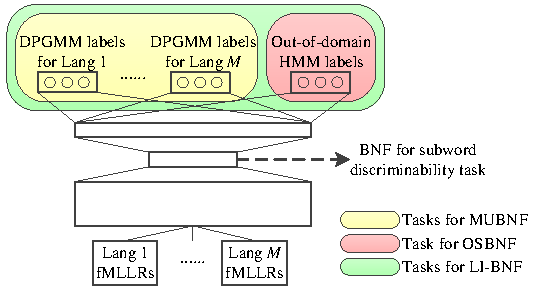
\includegraphics[width = 0.8 \linewidth]{MTL_tnr_embed.pdf}
\caption{DNN for extracting LI-BNF, MUBNF and OSBNF}
\label{fig:mtl}
\end{figure}
There are in total $M+1$ tasks, where $M$ denotes the number of target zero-resource languages. The first $M$ tasks predict language-dependent DPGMM labels for $M$ languages, while the additional language-independent task predicts HMM state labels generated by decoding results of an out-of-domain ASR system.
% out-of-domain ASR decoding results. 
Hidden layers, including a low-dimensional linear bottleneck layer, are shared between all target languages, while soft-max output layers are task-specific. After training, the language-independent BNFs (LI-BNFs) are used for subword discriminability task. Note that
 % in DNN-based feature representation learning framework, 
one could also choose either $M$ language-dependent tasks or the language-independent task for DNN training, and extract BNFs for evaluation. To differentiate from LI-BNFs, as illustrated in Figure \ref{fig:mtl}, in this paper BNFs extracted by a DNN trained in the former case is denoted as multilingual unsupervised  BNFs (MUBNFs), while  in the latter case is denoted as out-of-domain supervised BNFs (OSBNFs).
% , as can be referred in Figure \ref{fig:mtl}.
% either $M$ language-dependent tasks and or the language-independent task could 

There are two main reasons for us to perform MTL instead of single-task learning (STL). 
First, there are two frame labeling approaches investigated in this work, one based on DPGMM, the other based on an out-of-domain ASR.
% , of which one is language-dependent DPGMM label, the other is language-mismatched HMM state label by out-of-domain ASR decoding result. 
The tasks of predicting two types of labels are believed to be positively correlated, which satisfies the requirements of benefiting from MTL \cite{caruana1998multitask}.
Second, one requirement of the challenge 2017 is that the learned feature representation for all target languages be generated by the exact same system input-output. The idea of training a separate DNN for each target language is on the contrary with this\footnote{\label{footnote:ffnn}Although better  performance was found by language-specific BNFs during our experiments, we do not report it in this paper.}. 

\section{System fusion}
If multiple feature representation learning systems provide complementary information for target speech subword discriminability, fusion of these systems is believed to improve feature representation capability.
 % for subword discriminability task. 
System fusion can be made in different levels, e.g., model-level and output-level. MTL is one kind of model-level system fusion, as it composes several STL or MTL sub-systems. LI-BNFs, as described in Section \ref{sec:MTL}, can be considered as model-level fusion of MUBNFs and OSBNFs. Output-level system fusion is realized by directly concatenating features for the same speech frame extracted by multiple original systems. 
% The dimension of output-level fused features are the sum of original learned feature dimensions. 
In this work, the effectiveness of output-level system fusion is validated by concatenating language-mismatched BNFs (LM-BNFs), which are extracted by an out-of-domain DNN-HMM AM, and  LI-BNFs, or concatenating LM-BNFs, MUBNFs and OSBNFs together. 
% The effectiveness   of concatenating BNFs extracted by both in-domain and out-of-domain trained DNNs is 
% Both model-level and output-level system fusion methods are explored in this work.

\section{Experiments}

\subsection{Dataset and evaluation metric}
% To evaluate our methods of unsupervised feature representation learning, and to facilitate direct comparison between our system and state-of-the-art works by other researchers, the 
Experiments are carried out with development data of ZeroSpeech 2017 track one \cite{dunbar2017zero}.
% , \textit{unsupervised subword modeling} task \cite{dunbar2017zero}. 
The development data consists of three languages, i.e., English, French and Mandarin. Each language contains separate training and test sets of un-transcribed speech. Speaker identities are made publicly known for train sets while unknown for test sets. Test utterances lie in one of three lengths, 1s, 10s and 120s. Detailed information of data is listed in Table \ref{tab:zr17_data}.

\begin{table}[htbp]
\renewcommand\arraystretch{0.8}
\centering
\caption{Development data in ZeroSpeech 2017 track one}
\resizebox{0.65 \linewidth}{!}{%
\begin{tabular}{lcc|c}      
% \hline      
\toprule
 & \multicolumn{2}{c|}{ Training} & Test \\
\midrule
 & Duration & \#speakers  & Duration\\
% \hline
\midrule
English & 45 hrs & 60 & 27 hrs\\
French & 24 hrs & 18 & 18 hrs\\
Mandarin & 2.5 hrs & 8 & 6 hrs\\
% Training hours:  & $19.3$ & $81.5$ & $105.3$ \\
% Test hours:& $0.6$ & $0.7$ & $5.9$ \\
% Basic acoustic unit:  & Phone & Phone & Initial-Final \\
% \#basic units (inc. sil):& $33$ & $87$ & $61$ \\
% \#tied CD-HMM states:& $2462$ & $3431$ & $2386$ \\ 
% Lexicon size:& $ $ & $ 133K$& $ $ \\
% $\#$ Phonemes: &$43$& $46$&$ 29$& $44$& $38$\\
% \hline
\bottomrule
\end{tabular}%
}
\label{tab:zr17_data}
\end{table}

The evaluation metric of ZeroSpeech 2017 is ABX subword discriminability. Briefly speaking, the ABX task is to decide whether $X$ belongs to $x$ or $y$ if $A$ belongs to $x$ and $B$ belongs to $y$, where $A$, $B$ and $X$ are three speech segments, $x$ and $y$ are two phonemes that differ in the central sound (e.g., \quotes{beg}-\quotes{bag}, etc). 
% Dynamic time warping (DTW) is used to measure the dissimilarity between each pair of speech segments, the underlying frame-level dissimilarity is allowed to be defined by participants. In this paper, cosine distance is selected as recommended by challenge organizers. 
Each pair of segments $A$ and $B$ belong to the same speaker. 
% Depending on whether the segment $X$ belongs to the same speaker as $A$($B$), 
ABX error rates for \textit{within-talker} and \textit{across-talker} are evaluated separately, depending on whether $X$ belongs to the same speaker as $A(B)$.
Dynamic time warping (DTW) and cosine distance are used to measure segment-level and frame-level dissimilarity, respectively.
% More details can be found on \cite{dunbar2017zero}.

\subsection{Out-of-domain ASR system}
\label{subsec:ood_asr}
A Cantonese ASR is selected as the out-of-domain ASR system. 
% We choose Cantonese as a resource-rich language for two main reasons. First, Cantonese is different from any languages in ZeroSpeech 2017 development data, in line with the spirit of unsupervised learning. 
% It is worth noting that although both  Mandarin and Cantonese belong to Chinese, these two languages are mutually unintelligible. 
% A well-developed Cantonese ASR system has been trained in our previous work, which facilitates the system design in this work. 
The ASR is trained with CUSENT, a read speech corpus developed by The Chinese University of Hong Kong \cite{LeeLoChingEtAl2002}. There are $20,378$ training utterances from $34$ male and $34$ female speakers, with total $19.3$ hours data size. Kaldi \cite{povey2011kaldi} is used to train two versions of acoustic models, one is CD-GMM-HMM-SAT, the other is DNN-HMM.  
DNN-HMM is trained with alignment generated by CD-GMM-HMM-SAT model.
% and a syllable trigram language model. 
Input features are $40$-dimensional fMLLRs for CD-GMM-HMM-SAT model, or fMLLRs by splicing with context size $\pm 5$ for DNN-HMM. The fMLLR features are estimated by firstly performing VTLN towards $39$-dimensional MFCCs+$\Delta$+$\Delta\Delta$, followed by splicing with context size $\pm 3$ to estimate $40$-dimensional LDA and MLLT, followed by fMLLR estimation. The total number of CD-HMM states are $2462$. DNN-HMM has $7$ hidden layers, with dimensions $440$-$1024\times 5$-$40$-$1024$-$2462$. Sigmoid  is chosen as nonlinear activation function.
% The nonlinear function is Sigmoid, except for the linear bottleneck layer. 
A syllable trigram LM is trained with CUSENT training data transcription by SRILM \cite{Stolcke02srilm--}.
\begin{table*}[htbp]
\renewcommand\arraystretch{0.75}
\centering
\caption{ABX error rate ($\%$) on the proposed methods, MFCC and state of the art of ZeroSpeech 2017}
\resizebox{1 \linewidth}{!}{%
\begin{tabular}{lccc|ccc|ccc|c||ccc|ccc|ccc|c||c}      
% \hline      
\toprule
 & \multicolumn{10}{c||}{ Within-talker} & \multicolumn{10}{c||}{ Across-talker} & Avg.\\
\midrule
 & \multicolumn{3}{c|}{ English} & \multicolumn{3}{c|}{ French} & \multicolumn{3}{c|}{Mandarin}& Avg.&\multicolumn{3}{c|}{ English} & \multicolumn{3}{c|}{ French} & \multicolumn{3}{c|}{Mandarin} & Avg.\\
 & 1s & 10s & 120s & 1s & 10s & 120s & 1s & 10s & 120s && 1s & 10s & 120s & 1s & 10s & 120s & 1s & 10s & 120s &\\ 
% \midrule
%  & Duration & \#speakers  & Duration\\
% \hline
\midrule
Baseline (MFCC) \cite{dunbar2017zero}& 12.0 & 12.1 & 12.1 & 12.5 &12.6 &12.6 &11.5 &11.5 & 11.5&12.0 & 23.4& 23.4& 23.4& 25.2&25.5 &25.2 &21.3 &21.3 &21.3 & 23.3 & 17.7\\

fMLLR & 8.0 & 8.2 & 7.3 & 10.3 & 10.3 & 9.1 & 9.3 & 9.3 & 8.4 & 8.9 & 13.4 & 12.0 & 11.3 & 17.2 & 15.8 & 14.8 & 10.7 & 10.2 & 9.4 & 12.8 & 10.8 \\

MUBNF & 7.4 & 6.9 & 6.3 & 9.6 & 9.0 & 8.1 & 9.8 & 8.8 & 8.1 & 8.2 & 10.9 & 9.5 & 8.9 & 15.2 & 13.0 & 12.0 & 10.5 & 8.9 & 8.2 & 10.8 & 9.5\\

OSBNF & 7.2 &7.1&6.3&10.2&9.7& 8.7&9.1 &8.6 &7.6 & 8.3 & 10.0& 9.7&8.6&13.9&13.4&11.6&9.0&8.4&7.5&10.2&9.3\\

LI-BNF & 6.9 & 6.6 & 6.1 & 9.5 & 9.2 & 8.4 & 9.2 & 8.5 & 7.9 & 8.0 & 10.0 & \textbf{8.9} & \textbf{8.2} & 14.3 & 12.9& 11.5& 9.5& 8.5& 7.7 & 10.2 &9.1\\

LM-BNF & 7.2 & 6.8& 6.1& 9.6 & 9.0 & 8.0& 8.7& 7.6& 6.8& 7.8 & 10.6& 9.6& 8.7& 14.2& 13.2& 11.5& 8.5& \textbf{7.6}& \textbf{6.7}& 10.1& 8.9 \\

LM-BNF + LI-BNF & 7.0& 6.6& 6.0& 9.3& 8.8& 7.9& 8.6& \textbf{7.5}& \textbf{6.7}& 7.6& 10.3& 9.3& 8.4& 13.9& 12.9& 11.4& 8.5& \textbf{7.6}& \textbf{6.7}& 9.9& 8.7\\
LM-BNF + MUBNF + OSBNF & \textbf{6.8}& \textbf{6.4}& \textbf{5.8}& \textbf{9.0}& \textbf{8.8}& \textbf{7.8}& \textbf{8.5}& 7.7& 6.8& \textbf{7.5}& \textbf{9.9}& 9.0& \textbf{8.2}& \textbf{13.6}& \textbf{12.6}& \textbf{11.1}& \textbf{8.4}& 7.7& \textbf{6.7}& \textbf{9.7}& \textbf{8.6}\\
\midrule 
Heck et al. \cite{heck2017feature} & 6.9 & 6.2 & 6.0 & 9.7 & 8.7 & 8.4 & 8.8 & 7.9 & 7.8 & 7.8 & 10.1 & 8.7 & 8.5 & 13.6 & 11.7 & 11.3 & 8.8 & 7.4 & 7.3 & 9.7 & 8.8\\

System 1, Shibata et al.  \cite{shibata2017composite} & 6.7 & 6.5 & 5.7 & 9.7 & 9.2 & 7.9 & 9.8 & 9.2 & 8.2 & 8.1 & 10.1 & 9.2 & 8.2 & 13.7 & 12.4 & 10.8 & 10.4 & 9.5 & 8.0 & 10.3 & 9.2 \\ 
% Topline  & 6.5& 6.3 & 5.1 & \\
 % & 2.5 hrs & 8 & 6 hrs\\
% Training hours:  & $19.3$ & $81.5$ & $105.3$ \\
% Test hours:& $0.6$ & $0.7$ & $5.9$ \\
% Basic acoustic unit:  & Phone & Phone & Initial-Final \\
% \#basic units (inc. sil):& $33$ & $87$ & $61$ \\
% \#tied CD-HMM states:& $2462$ & $3431$ & $2386$ \\ 
% Lexicon size:& $ $ & $ 133K$& $ $ \\
% $\#$ Phonemes: &$43$& $46$&$ 29$& $44$& $38$\\
% \hline
\bottomrule
\end{tabular}%
}
\label{tab:abx_results}
\end{table*}
\subsection{Speaker adaptation of target speech}
The Cantonese ASR is used to perform fMLLR-based speaker adaptation of target speech in a two-pass procedure. 
% Training sets of ZeroSpeech 2017 data are formed as one entire utterance for a specific speaker, and a few training utterances last for several hours. This is impractical to be decoded at one time. To cope with this problem, we simply segment training utterances to no longer than 10s for each segmented speech.  
In the first-pass, target speech is decoded by the ASR in a speaker-independent manner using unadapted features, from which initial fMLLR transforms are estimated. 
% Speaker adaptation statistics is then collected and used to estimate initial fMLLR transforms. 
In the second-pass, target speech features transformed by the initial fMLLRs are decoded by the ASR in a speaker-adaptive manner. Finally the fMLLR transforms for the target speech are estimated.
\subsection{Frame labeling and MTL-DNN training}
Two frame labeling approaches are implemented. DPGMM clustering based frame labeling for target unsupervised speech is implemented using tools developed by Chang et al. \cite{chang2013parallel}. The features used in clustering are $40$-dimensional fMLLRs for ZeroSpeech 2017 training sets. Frames of each language are clustered individually. 
% The cluster number does not need to be defined in prior. 
Clustering iterations for English, French and Mandarin corpora are $120, 200$ and $3000$, resulting in cluster numbers $1118, 1345$ and $596$, respectively. After training, each frame is assigned with a DPGMM label.
On the other hand, the out-of-domain ASR based frame labeling is implemented by decoding target speech of three languages using the Cantonese DNN-HMM ASR.
% using the Cantonese DNN-HMM ASR system described in Section \ref{subsec:ood_asr}. Target speech of all three languages are decoded by the ASR. 
After decoding, lattices are converted to one best path for each utterance, with LM to AM weight ratio set to $0.001$. Each best path comprises a sequence of CD-HMM states defined in AM of the Cantonese ASR. These CD-HMM states are regarded as out-of-domain ASR based frame labels.

MTL-DNN is trained with $40$-dimensional fMLLRs with context size $\pm 5$ for training sets of three languages. There are $4$ equally weighted tasks in MTL, $3$ language-dependent DPGMM label prediction tasks and a language-mismatched Cantonese CD-HMM state prediction task. The NN structure is 
% $440$-$1024\times 5$-$40$-$1024$-$\mathrm{<Block\textrm{ }softmax>}$, 
$440$-$1024\times 5$-$40$-$1024$-\quotes{Block softmax layers},
where block softmax layer dimensions for $4$ tasks are $1118, 1345, 596$ and $2462$, in sequence. After MTL-DNN training, $40$-dimensional language-independent BNFs (LI-BNFs) for test sets of three languages are extracted and used for ABX task. Similarly, multilingual unsupervised BNFs (MUBNFs), extracted by MTL-DNN with only first $3$ DPGMM label prediction tasks, and out-of-domain supervised BNFs (OSBNFs), extracted by STL-DNN with only the Cantonese CD-HMM state prediction task, are also used for ABX task. The dimensions of both MUBNFs and OSBNFs are $40$.
\subsection{System fusion}
For model-level system fusion approach, LI-BNFs can be regarded as a fusion of MUBNFs and OSBNFs. For output-level system fusion approach, two configurations are made, i.e., appending LM-BNFs to LI-BNFs, resulting in $80$-dimensional features, and concatenating LM-BNFs, MUBNFs and OSBNFs together, resulting in $120$-dimensional features. LM-BNFs are extracted by feeding forward fMLLRs of ZeroSpeech 2017 test sets to bottleneck layer of Cantonese DNN-HMM AM. Attributes of the concerned BNFs  
% LI-BNF, MUBNF, OSBNF and LM-BNF 
are listed in Table \ref{tab:bnf_attrib}. 
\begin{table}[htbp]
\renewcommand\arraystretch{0.9}
\centering
\caption{Attributes of LM-BNF, MUBNF, OSBNF and LM-BNF}
\resizebox{0.9 \linewidth}{!}{%
\begin{tabular}{l|c|c|c|c}      
% \hline      
\toprule
& LI-BNF & MUBNF & OSBNF & LM-BNF \\
\midrule
Training method & MTL & MTL & STL & STL \\
\midrule
Training data & \multicolumn{3}{c|}{ZeroSpeech 2017 fMLLR} & CUSENT fMLLR\\
\midrule 
Label type & Sup. \& Unsup. & Unsup. & Sup. & Sup. \\
\midrule
Dimension & \multicolumn{4}{c}{40} \\
% \hline
% \midrule
% Labels & DPGMM \& \\
% Training hours:  & $19.3$ & $81.5$ & $105.3$ \\
% Test hours:& $0.6$ & $0.7$ & $5.9$ \\
% Basic acoustic unit:  & Phone & Phone & Initial-Final \\
% \#basic units (inc. sil):& $33$ & $87$ & $61$ \\
% \#tied CD-HMM states:& $2462$ & $3431$ & $2386$ \\ 
% Lexicon size:& $ $ & $ 133K$& $ $ \\
% $\#$ Phonemes: &$43$& $46$&$ 29$& $44$& $38$\\
% \hline
\bottomrule
\end{tabular}%
}
\label{tab:bnf_attrib}
\end{table}
In this Table, unsupervised DPGMM labels are denoted as \quotes{Unsup.}, while Cantonese CD-HMM state labels are denoted as \quotes{Sup.}.


% This is the discussion. This is the discussion. This is the discussion. Is there any discussion?

% \cite{Wang2014}\cite{ansari2017deep}\cite{ansari2017unsupervised}\cite{heck2017feature}\cite{shibata2017composite}\cite{yuan2017extracting}\cite{chen2017multilingual}

\section{Results and analyses}
Experimental results of our proposed methods and state of the art of ZeroSpeech 2017 are summarized in Table \ref{tab:abx_results}. Baseline (MFCC) is released by challenge organizers. The sign \quotes{+} in Table \ref{tab:abx_results} denotes output-level system fusion by feature concatenation. From this Table, several observations are made.

(1) FMLLR features consistently outperform MFCCs on all target languages, reducing   average ABX  error rates with relative 33.3\% and 45.1\% in within-talker and across-talker evaluation conditions, respectively. At this stage training sets of ZeroSpeech 2017 are not used. Speaker adaptation based on an out-of-domain ASR system is effective and efficient for unsupervised subword modeling. The learned fMLLRs
% Table \ref{tab:abx_results} also shows that compared with MFCCs, the learned fMLLR features 
achieve more ABX error rate reduction on long test utterances than on short ones. This is probably because fMLLR-based speaker adaptation does not work well on very short speech. 
 % {\color{red}{draw a bar figure to explicitly compare 1s 10s 120s}}

% Even without using any training sets of target speech, 
(2) MTL-DNN training with fMLLR features followed by system fusion  bring the best performance. LI-BNFs, trained with both DPGMM labels and out-of-domain HMM state labels, 
% $3$ language-dependent DPGMM label prediction tasks and $1$ out-of-domain HMM state label prediction task, 
reduce within and across-talker average ABX error rates by relative 10.1\% and 20.3\%, as compared with fMLLRs. Our best system concatenates LM-BNFs, MUBNFs and OSBNFs and achieves 7.5\%/9.7\% average ABX error rates in within/across-talker conditions, which is highly competitive  with the best submitted system for the challenge  by Heck et al. \cite{heck2017feature} (7.8\%/9.7\%). It must be noted that system development in \cite{heck2017feature} does not rely on any out-of-domain  resources, while our system uses $19.3$ hours Cantonese transcribed speech. Our best system outperforms System $1$ of Shibata et al. \cite{shibata2017composite} (8.1\%/10.3\%) in both 
% in which around $240$ hours Japanese transcribed speech are used in ASR development 
% within and across-talker 
conditions. Note that \cite{shibata2017composite} uses $240$ hours Japanese transcribed speech in System 1 development. 
% in which around $240$ hours Japanese transcribed speech are used in ASR development 
% within and across-talker evaluation conditions.
% , the performance of which is directly comparable to ours.

(3) Better unsupervised feature representation can be learned when the combination of in-domain and out-of-domain resources is realized by any of model and output-level system fusion.  
% To learn better feature representation of unsupervised speech, the idea of combining in-domain and out-of-domain resources could be realized by both model and output-level system fusion.
% combining different methods of exploiting out-of-domain transcribed and speaker annotated data lead to better performance. 
Compared with MUBNF, the advantage of LI-BNF is probably because the additional task of predicting out-of-domain CD-HMM state labels serves as supplement to in-domain DPGMM label prediction tasks. DPGMM labels are generated in an unsupervised, purely data-driven manner, whilst out-of-domain CD-HMM state labels regularize in-domain data in a phonetically-aware form. On the other hand, LM-BNF, extracted by an out-of-domain DNN, gives compact language-mismatched phonetically-discriminative representation.  By concatenating LM-BNFs, MUBNFs and OSBNFs, phonetically-discriminative information in both domains is combined and lead to better  feature representation than any one of LM-BNFs, MUBNFs and OSBNFs.

\section{Conclusions}
This paper presents a study on exploiting knowledge from resource-rich languages for unsupervised feature representation learning of zero-resource speech. Out-of-domain transcribed and speaker annotated speech is employed to perform speaker adaptation towards zero-resource speech. Frame labeling methods including DPGMM clustering and out-of-domain ASR decoding are adopted to provide supervision for multi-task learning DNN (MTL-DNN) training. Bottleneck features (BNFs) extracted by MTL-DNN are used for ABX subword discriminability task. Moreover, system fusion is performed by concatenating BNFs extracted by in-domain and out-of-domain trained DNNs.
% language-mismatched BNFs (LM-BNFs) and in-domain DNN extracted BNFs.
 % extracted by an out-of-domain DNN  are concatenated 
Experiments are carried out with Zero Resource Speech Challenge 2017 track one. Experimental results show that: (1) Speaker adaptation based on out-of-domain ASR system is effective and efficient; (2) Our best system achieves highly competitive performance to state of the art; (3) Model and output-level system fusion methods both improve subword discriminability of the learned feature representation. 

% ABX task performance could be improved by different strategies of combining in-domain and out-of-domain resources. Model-level fusion by MTL with in-domain and out-of-domain label prediction, output-level fusion by concatenating BNFs extracted by in-domain and out-of-domain trained DNNs.
% provide complementary supervision for subword discriminative learning of feature representation. 
% Authors must proofread their PDF file prior to submission to ensure it is correct. Authors should not rely on proofreading the Word file. Please proofread the PDF file before it is submitted.

% \section{Acknowledgements}
% This research is partially supported by a GRF project grant (Ref: CUHK 14227216) from Hong Kong Research Grants Council.



% The ISCA Board would like to thank the organizing committees of the past INTERSPEECH conferences for their help and for kindly providing the template files. \\
% Note to authors: Authors should not use logos in acknowledgement section; rather authors should acknowledge corporations by naming them only.

% \newpage
\bibliographystyle{IEEEtran}

\bibliography{mybib.bib}

% \begin{thebibliography}{9}
% \bibitem[1]{Davis80-COP}
%   S.\ B.\ Davis and P.\ Mermelstein,
%   ``Comparison of parametric representation for monosyllabic word recognition in continuously spoken sentences,''
%   \textit{IEEE Transactions on Acoustics, Speech and Signal Processing}, vol.~28, no.~4, pp.~357--366, 1980.
% \bibitem[2]{Rabiner89-ATO}
%   L.\ R.\ Rabiner,
%   ``A tutorial on hidden Markov models and selected applications in speech recognition,''
%   \textit{Proceedings of the IEEE}, vol.~77, no.~2, pp.~257-286, 1989.
% \bibitem[3]{Hastie09-TEO}
%   T.\ Hastie, R.\ Tibshirani, and J.\ Friedman,
%   \textit{The Elements of Statistical Learning -- Data Mining, Inference, and Prediction}.
%   New York: Springer, 2009.
% \bibitem[4]{YourName17-XXX}
%   F.\ Lastname1, F.\ Lastname2, and F.\ Lastname3,
%   ``Title of your INTERSPEECH 2018 publication,''
%   in \textit{Interspeech 2018 -- 19\textsuperscript{th} Annual Conference of the International Speech Communication Association, September 2-6, Hyderabad, India Proceedings, Proceedings}, 2018, pp.~100--104.
% \end{thebibliography}

\end{document}
